\documentclass[border=4pt]{standalone}
\usepackage{amsmath,amssymb}
\usepackage{tikz}
\usetikzlibrary{arrows.meta,positioning,shapes.geometric,calc}
\begin{document}
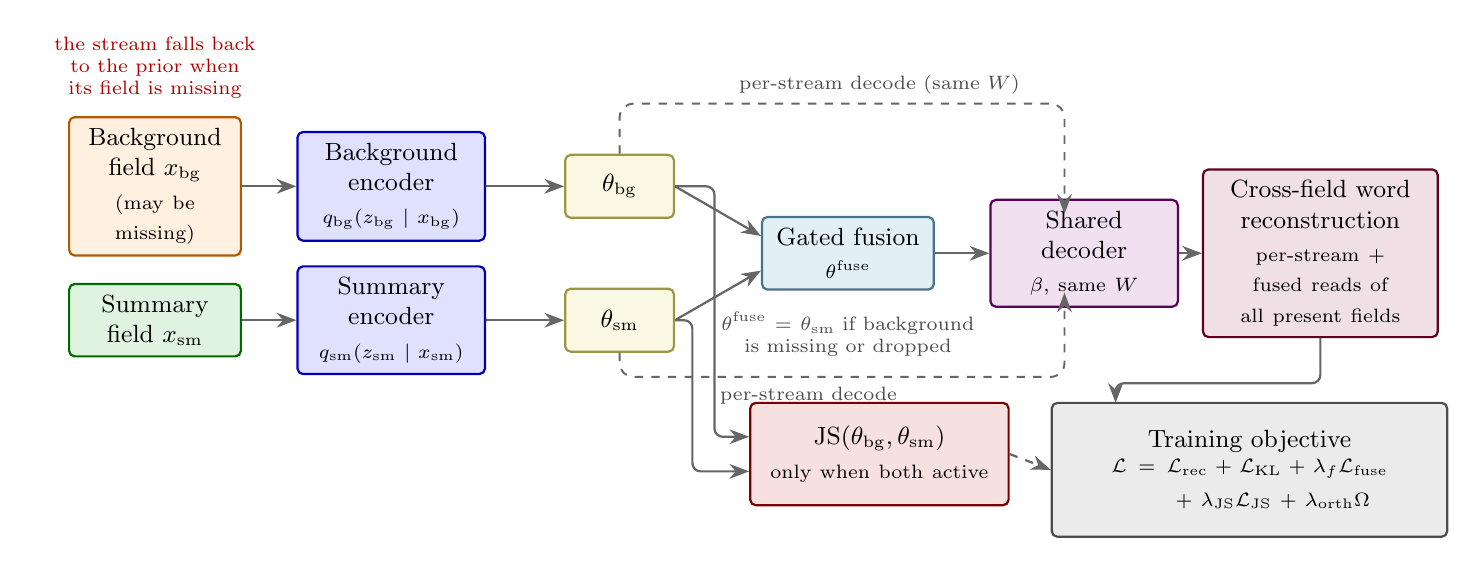
\begin{tikzpicture}[
  font=\small,
  box/.style={draw=#1!70!black, fill=#1!12, rounded corners=2pt, align=center,
              inner sep=4pt, minimum height=8mm, line width=0.8pt},
  arrow/.style={-{Stealth[length=2.5mm]}, line width=0.8pt, color=black!60},
  darrow/.style={-{Stealth[length=2.5mm]}, line width=0.7pt, color=black!60, dashed},
  lab/.style={font=\scriptsize, color=black!70}
]
\node[box=orange, text width=19mm] (rc) at (0,0) {Background field $x_{\mathrm{bg}}$\\[1pt]{\scriptsize (may be missing)}};
\node[box=green!60!black, text width=19mm] (ri) at (0,-1.7) {Summary field $x_{\mathrm{sm}}$};
\node[box=blue, text width=21mm] (ec) at (3.0,0) {Background encoder\\[1pt]{\scriptsize $q_{\mathrm{bg}}(z_{\mathrm{bg}}\mid x_{\mathrm{bg}})$}};
\node[box=blue, text width=21mm] (ei) at (3.0,-1.7) {Summary encoder\\[1pt]{\scriptsize $q_{\mathrm{sm}}(z_{\mathrm{sm}}\mid x_{\mathrm{sm}})$}};
\node[box=yellow!80!black, text width=11mm] (tc) at (5.9,0) {$\theta_{\mathrm{bg}}$};
\node[box=yellow!80!black, text width=11mm] (ti) at (5.9,-1.7) {$\theta_{\mathrm{sm}}$};
\node[box=cyan!70!black, text width=19mm] (fuse) at (8.8,-0.85) {Gated fusion\\[1pt]{\scriptsize $\theta^{\mathrm{fuse}}$}};
\node[box=violet, text width=21mm] (dec) at (11.8,-0.85) {Shared decoder\\[1pt]{\scriptsize $\beta$, same $W$}};
\node[box=purple!70!black, text width=27mm] (rec) at (14.8,-0.85) {Cross-field word reconstruction\\[1pt]{\scriptsize per-stream $+$ fused reads of all present fields}};
\node[box=red!70!black, text width=30mm, minimum height=13mm] (js) at (9.2,-3.4) {JS$(\theta_{\mathrm{bg}},\theta_{\mathrm{sm}})$\\[1pt]{\scriptsize only when both active}};
\node[draw=black!70, fill=black!8, rounded corners=2pt, align=center, inner sep=6pt,
      minimum height=17mm, line width=0.8pt, text width=46mm] (loss) at (13.9,-3.6)
      {Training objective\\[1pt]{\scriptsize
       $\mathcal{L}=\mathcal{L}_{\mathrm{rec}}+\mathcal{L}_{\mathrm{KL}}+\lambda_f\mathcal{L}_{\mathrm{fuse}}$\\[1pt]
       $\phantom{\mathcal{L}=}+\lambda_{\mathrm{JS}}\mathcal{L}_{\mathrm{JS}}+\lambda_{\mathrm{orth}}\Omega$}};
\draw[arrow] (rc) -- (ec);
\draw[arrow] (ri) -- (ei);
\draw[arrow] (ec) -- (tc);
\draw[arrow] (ei) -- (ti);
\draw[arrow] (tc.east) -- ([yshift=2.2mm]fuse.west);
\draw[arrow] (ti.east) -- ([yshift=-2.2mm]fuse.west);
\draw[arrow] (fuse.east) -- (dec.west);
\draw[arrow] (dec.east) -- (rec.west);
\draw[darrow, rounded corners=5pt] (tc.north) -- (5.9,1.05) -- (11.55,1.05) -- (11.55,-0.35);
\node[lab, above] at (9.2,1.05) {per-stream decode (same $W$)};
\draw[darrow, rounded corners=5pt] (ti.south) -- (5.9,-2.42) -- (11.55,-2.42) -- (11.55,-1.35);
\node[lab, below] at (8.3,-2.42) {per-stream decode};
\draw[arrow, rounded corners=3pt] (tc.east) -- ++(0.50,0) |- ([yshift=2.2mm]js.west);
\draw[arrow, rounded corners=3pt] (ti.east) -- ++(0.22,0) |- ([yshift=-2.2mm]js.west);
\draw[arrow, rounded corners=3pt] (rec.south) -- (14.8,-2.5) -- (12.2,-2.5) -- (12.2,-2.75);
\draw[arrow, dashed] (js.east) -- (loss.west);
\node[red!70!black, font=\scriptsize, above=1mm of rc, text width=30mm, align=center]
      {the stream falls back to the prior when its field is missing};
\node[lab, below=1.5mm of fuse, text width=36mm, align=center]
      {$\theta^{\mathrm{fuse}}=\theta_{\mathrm{sm}}$ if background is missing or dropped};
\end{tikzpicture}
\end{document}
